\begin{frame}{Build a neural network: target and inputs?}

\begin{minipage}[c]{.49\textwidth}
\manip Model target: generated Higgs mass.
\manip Model inputs:
\submanip $\tau_1$ (here = \muon) and $\tau_2$ (here = \tauh) $\pT, \eta, \phi$;
\submanip PuppiMET $\pT, \phi$;
\submanip METcov xx, xy and yy;
\submanip Number of neutrinos from \emph{reco} tau decays;
\submanip $\mT^{(1,MET)}$, $\mT^{(2,MET)}$, $\mT^{(1,2)}$, \mTtot\ (Puppi);
\submanip jet 1, jet 2 $\pT, \eta, \phi$;
\submanip Additionnal Hadronic Activity $\pT, \eta, \phi$, \Njetsr;
\submanip \texttt{npvsGood} $\rightarrow$ how much PU.
\end{minipage}
\hfill
\begin{minipage}[c]{.48\textwidth}
\begin{block}{$\gluon\gluon\to\Higgs\to\tau\tau\to\mu\tauh$}
\begin{center}

\vspace{2\baselineskip}

\begin{fmffile}{H-tautau_mutau_small}\fmfstraight
\begin{fmfchar*}(50,25)
  \fmfleft{a,g1,b,c,g2,d}
  \fmfright{nu1,upq,doq,muout,antinumu,nu2}
  
  \fmf{gluon}{g1,g1loop}
  \fmf{gluon}{g2,g2loop}
  \fmf{phantom, tension=.2}{g1loop,upq}
  \fmf{phantom, tension=.2}{g2loop,antinumu}
  \fmffreeze
  \fmf{fermion}{g1loop,hloop,g2loop,g1loop}
  \fmf{fermion}{g2loop,g1loop}
  \fmf{dashes, label=$\Hn$, l.side=left, tension=1}{hloop,v}
  \fmf{phantom, tension=.2}{nu1,v,nu2}
  \fmffreeze
  
  \fmf{fermion, label=$\antitau$, l.side=left, tension=4}{t1d,v}
  \fmf{fermion, label=$\leptau$, l.side=left, tension=4}{v,t2d}
  \fmf{fermion, tension=3}{nu1,t1d}
  \fmf{boson, l.side=left, tension=2}{t1d,W1d}
  \fmf{phantom}{doq,W1d,upq}
  \fmf{fermion, tension=3}{t2d,nu2}
  \fmf{boson, tension=2}{t2d,W2d}
  \fmf{fermion}{antinumu,W2d,muout}
  \fmffreeze
  \fmf{plain}{W1d,upq}
  
  \fmflabel{\gluon}{g1}
  \fmflabel{\gluon}{g2}
  
  \fmflabel{{\color{ltcolorgray2}$\antinutau$}}{nu1}
  \fmflabel{{\color{ltcolorgray2}$\nutau$}}{nu2}
  \fmflabel{{\color{\muoncolor}$\muon$}}{muout}
  \fmflabel{{\color{ltcolorgray2}$\antinumu$}}{antinumu}
  \fmflabel{{\color{\tauhcolor}$\tauh$}}{upq}
  \fmfdot{g1loop,hloop,g2loop,v,t1d,t2d,W2d}
  \fmfblob{.07w}{W1d}
\end{fmfchar*}
\end{fmffile}


\vspace{2\baselineskip}

\end{center}
\end{block}
\end{minipage}

\vfill

\begin{equation*}
\boxed{\mTtot = \sqrt{\mT^2(\tau_1,\MET) + \mT^2(\tau_2,\MET) + \mT^2(\tau_1,\tau_2)}}
\msep
\mT(1,2) = \sqrt{2p_T^{(1)} p_T^{(2)} (1-\cos\Delta\phi)}
\end{equation*}

\end{frame}

\begin{frame}{Build a neural network: hyperparameters?}

\manip NN hyperparameters (and other tested values):
% NN-activation-softplus-batch_size-2048-mape-Adam-gu-inclusive-3-layers-1000-neurons
\submanip \textbf{Adam} optimizer (Adadelta, SGD),
\submanip Weight initialized with \textbf{Glorot uniform} (Glorot normal, normal, uniform),
\submanip Custom \LossMAPEsqrtb\ loss (\LossMAPE, \LossMAE, \LossMSE),
\submanip \textbf{Softplus} activation function (ReLU, ELU, SELU, Exponential),
\begin{equation*}
\mathit{softplus}(x) = \ln(1+\eexp{x})
\end{equation*}
\submanip \textbf{3} hidden layers (2 to 5),
\submanip \textbf{1000} neurons per hidden layer (200 to 2000 per steps of 100).
\end{frame}

\begin{frame}{Datasets?}

\begin{minipage}[c]{.49\textwidth}
\manip Generate $\higgsML\to\tau\tau$ events:
\submanip $\higgsML$ is SM Higgs (pdg ID 25) with a different mass,
\submanip \higgsML\ produced by gluon fusion,
\submanip set $\BR(\higgsML\to\tau\tau)=1$ to avoid non di-\tau\ events.

\manip All final states used simultaneously for training:
\submanip \tauh\tauh, \mu\tauh, \ele\tauh, \mu\mu, \ele\mu, \ele\ele.
\end{minipage}
\hfill
\begin{minipage}[c]{.48\textwidth}
\def\Higgs{\higgsML}
\begin{block}{$\gluon\gluon\to\Higgs\to\tau\tau\to\mu\tauh$}
\begin{center}

\vspace{2\baselineskip}

\begin{fmffile}{H-tautau_mutau_small}\fmfstraight
\begin{fmfchar*}(50,25)
  \fmfleft{a,g1,b,c,g2,d}
  \fmfright{nu1,upq,doq,muout,antinumu,nu2}
  
  \fmf{gluon}{g1,g1loop}
  \fmf{gluon}{g2,g2loop}
  \fmf{phantom, tension=.2}{g1loop,upq}
  \fmf{phantom, tension=.2}{g2loop,antinumu}
  \fmffreeze
  \fmf{fermion}{g1loop,hloop,g2loop,g1loop}
  \fmf{fermion}{g2loop,g1loop}
  \fmf{dashes, label=$\Hn$, l.side=left, tension=1}{hloop,v}
  \fmf{phantom, tension=.2}{nu1,v,nu2}
  \fmffreeze
  
  \fmf{fermion, label=$\antitau$, l.side=left, tension=4}{t1d,v}
  \fmf{fermion, label=$\leptau$, l.side=left, tension=4}{v,t2d}
  \fmf{fermion, tension=3}{nu1,t1d}
  \fmf{boson, l.side=left, tension=2}{t1d,W1d}
  \fmf{phantom}{doq,W1d,upq}
  \fmf{fermion, tension=3}{t2d,nu2}
  \fmf{boson, tension=2}{t2d,W2d}
  \fmf{fermion}{antinumu,W2d,muout}
  \fmffreeze
  \fmf{plain}{W1d,upq}
  
  \fmflabel{\gluon}{g1}
  \fmflabel{\gluon}{g2}
  
  \fmflabel{{\color{ltcolorgray2}$\antinutau$}}{nu1}
  \fmflabel{{\color{ltcolorgray2}$\nutau$}}{nu2}
  \fmflabel{{\color{\muoncolor}$\muon$}}{muout}
  \fmflabel{{\color{ltcolorgray2}$\antinumu$}}{antinumu}
  \fmflabel{{\color{\tauhcolor}$\tauh$}}{upq}
  \fmfdot{g1loop,hloop,g2loop,v,t1d,t2d,W2d}
  \fmfblob{.07w}{W1d}
\end{fmfchar*}
\end{fmffile}


\vspace{2\baselineskip}

\end{center}
\end{block}
\end{minipage}
\end{frame}

\begin{frame}{Datasets: low mass boundary}

\begin{minipage}[c]{.45\textwidth}
\manip Event selection:
\submanip Same as in the MSSM \HAtoTauTau\ analysis,
\submanip Add \mu\mu\ and \ele\ele\ channels.
\manip Events amount drops at low mass:
\submanip due to \pT\ cuts,
\submanip go down to \SI{50}{\GeV} for $m_{\higgsML}$.
\end{minipage}
\hfill
\begin{minipage}[c]{.45\textwidth}
\begin{center}
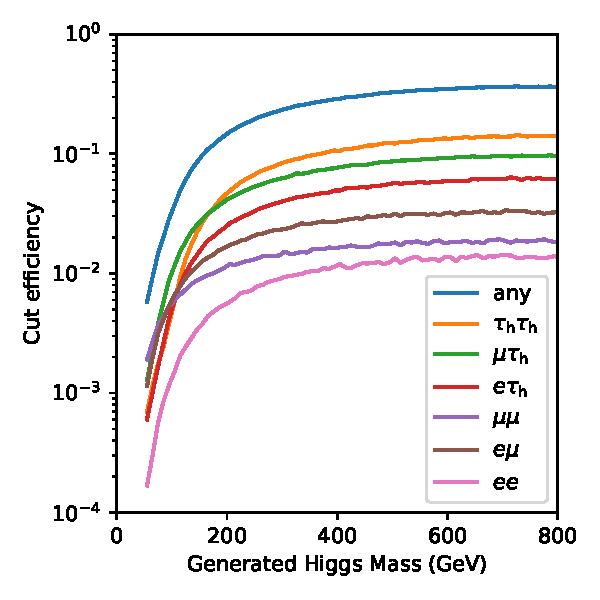
\includegraphics[width=\linewidth]{\PhDthesisdir/plots_and_images/my_plots/ML/from_ML_plots/FastSim_NanoAOD_to_NN/ALL_PU2017/plots_Htt_merged_NanoAODSIM_ALL_PU2017-DeepTau_1000/analysis_cuts_efficiency-en.pdf}
\end{center}
\end{minipage}

\begin{tikzpicture}[overlay, remember picture]
\draw [ltcolorred] (.2\textwidth, .15\textheight) node (A) {Less than \SI{1}{\%} pass the selection} ;

\draw [ltcolorred, thick] (.665\textwidth, .325\textheight) ellipse (.3 and 1.5);

\draw (.65\textwidth, .35\textheight) coordinate (B);
\draw [ltcolorred, thick, -latex] (A.east) to [out = 0, in = -170] (B);
\end{tikzpicture}
\end{frame}

\begin{frame}{Datasets: high mass boundary}

\beamercite{Higgs_xsec_book_3}
\begin{minipage}[c]{.52\textwidth}
\manip Higgs width $\simeq$ Higgs mass \tikzmarknode{around \SI{1}{\TeV}:}{A}
\submanip can't have coherent mass points using \higgsML,
\submanip go up to \SI{800}{\GeV} for $m_{\higgsML}$.

\manip Side note:
\submanip one can get higher mass points using \Higgs\ and \HiggsA,
\submanip we tried to extend the mass range without success,
\submanip \SI{800}{\GeV} large enough for \SI{13}{\TeV} \proton\proton\ collisions.
\end{minipage}
\hfill
\begin{minipage}[c]{.45\textwidth}
\vspace{-\baselineskip}
\begin{center}
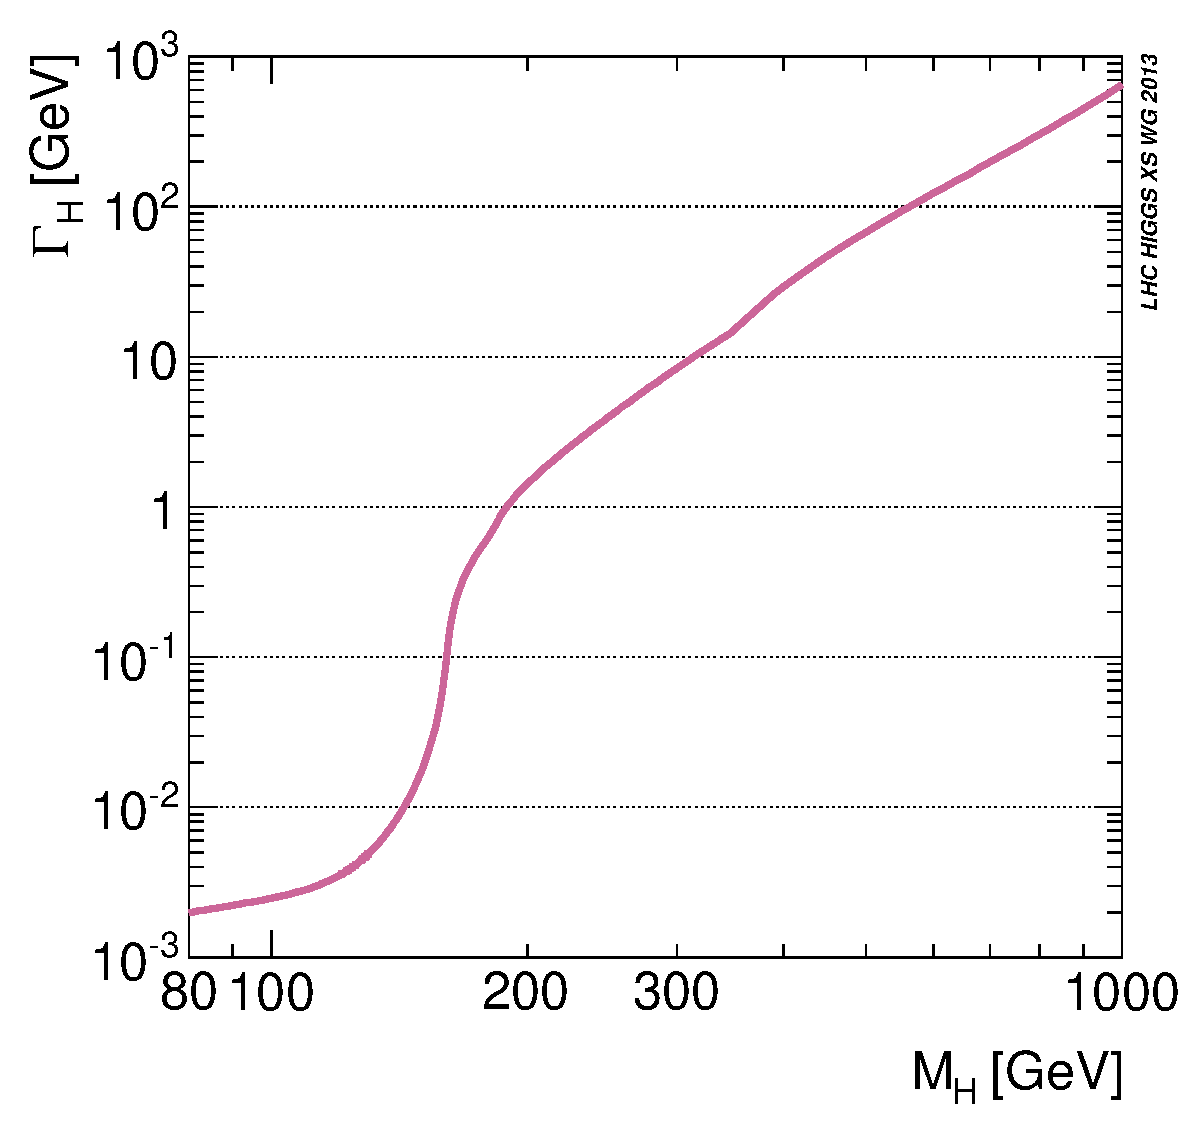
\includegraphics[width=\linewidth]{\PhDthesisdir/plots_and_images/from_Higgs_xsec_book_3/SM_Width.pdf}
\end{center}
\end{minipage}

\begin{tikzpicture}[overlay, remember picture]
%\draw [ltcolorred, thick] (.665\textwidth, .325\textheight) ellipse (.3 and 1.5);

\draw (.95\textwidth, .775\textheight) coordinate (B);
\draw [ltcolorred, thick, -latex] (A.east) to [out = 0, in = 175] (B);
\end{tikzpicture}
\end{frame}

\begin{frame}{DNN's \mml\ predictions \emph{vs} \mTtot}

\begin{minipage}[c]{.45\textwidth}
\only<1-2>{
\begin{center}
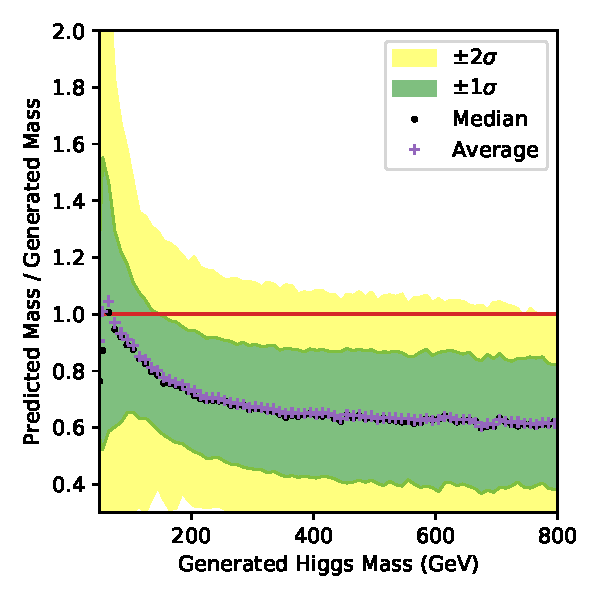
\includegraphics[width=\linewidth]{\PhDthesisdir/plots_and_images/my_plots/ML/from_ML_plots/FastSim_NanoAOD_to_NN/ALL_PU2017/plots_Htt_merged_NanoAODSIM_ALL_PU2017-DeepTau/model_response-PuppimTtot_reco-en.pdf}
\end{center}
}
\only<3->{
\manip $r=\num{1.00}\pm{0.05}$ from \num{80} to \SI{800}{\GeV}
\manip \higgsML\ mass reconstruction \textbf{achieved {\color{ltcolorgreen}\OK}}
}
\end{minipage}
\hfill
\begin{minipage}[c]{.45\textwidth}
\only<1>{
\manip Model's response:
\begin{equation*}
r = \frac{\text{prediction}}{\text{true value}} = \frac{\mml}{m_{\higgsML}} \text{ or } \frac{\mTtot}{m_{\higgsML}}
\end{equation*}
\manip Closer to 1 is better for black dots.
}
\only<2->{
\begin{center}
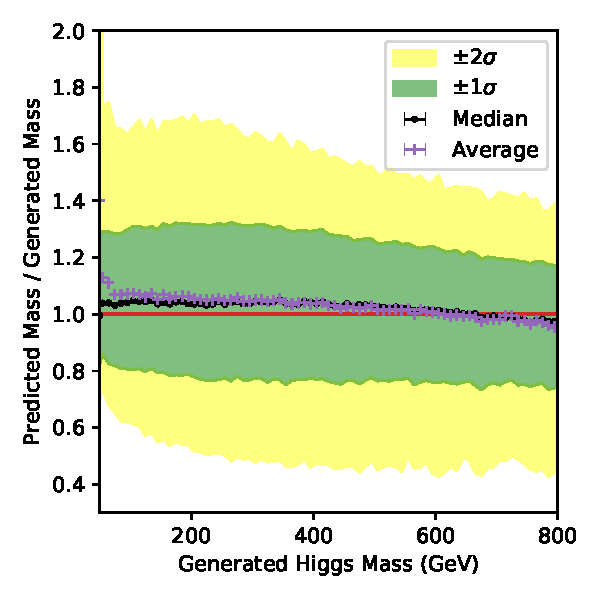
\includegraphics[width=\linewidth]{\PhDthesisdir/plots_and_images/my_plots/ML/from_ML_plots/selected_NNs_FastSim/DeepTau-inclusive-1TeV/PuppiMET_with_METcov_j1j2jr_Nnu_Npu/plots_up_to_800/model_response-NN-activation-softplus-batch_size-2048-mapesqrt_b-Adam-gu-inclusive-3-layers-1000-neurons-en.pdf}
\end{center}
}
\end{minipage}

\begin{tikzpicture}[overlay, remember picture]
\only<2>{\draw [ltcolorred] (.75\textwidth, .7\textheight) node {\Large DNN's \mml} ;}
\only<1-2>{\draw [ltcolorred] (.2\textwidth, .7\textheight) node {\Large\mTtot} ;}
\only<1>{
\draw [ltcolorred] (.2\textwidth, .6\textheight) node {\large completely off!} ;
\draw [ltcolorred] (.25\textwidth, .5\textheight) node {$\rightarrow$ not a good mass estimator.} ;
}
\end{tikzpicture}
\end{frame}

\begin{frame}{Using the model to get a discriminating variable}

\begin{minipage}[c]{.54\textwidth}
\manip In the \HAtoTauTau\ analysis, discriminating variable $=$ \mTtot.
\manip \mTtot\ is equal to the invariant mass assuming:
\submanip all neutrinos are a single particle with $\vpT = \vMET$,
\submanip all is going on in the transverse plane (any $p_z = 0$).

\manip \textbf{Our model has a better resolution} on $m_{\higgsML}$ than \mTtot.
\end{minipage}
\hfill
\begin{minipage}[c]{.45\textwidth}
\begin{center}
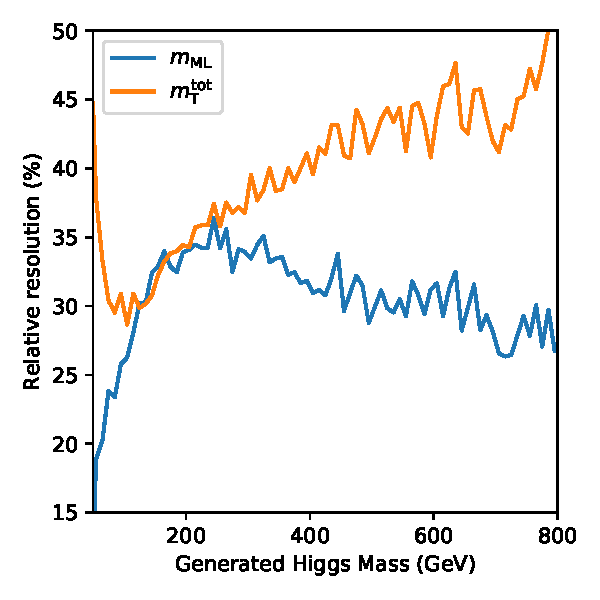
\includegraphics[width=\linewidth]{\PhDthesisdir/plots_and_images/my_plots/ML/from_ML_plots/selected_NNs_FastSim/DeepTau-inclusive-1TeV/PuppiMET_with_METcov_j1j2jr_Nnu_Npu/plots_up_to_800/model_relative_response-NN-activation-softplus-batch_size-2048-mapesqrt_b-Adam-gu-inclusive-3-layers-1000-neurons-en.pdf}
\end{center}
\end{minipage}

\end{frame}